\documentclass{article} 
\usepackage[utf8]{inputenc}
\usepackage[T1]{fontenc}
\usepackage{titling}
\newcommand{\inputparam}[2]{%
  \def\parg{#2}
  \input{#1}
}

\inputparam{intestazione}{Modello E-R}


\newpage

\section{Descrizione delle Entità e Attributi}
    \begin{itemize}[nosep, leftmargin=*]
        \item\textbf{USER (Utente):}
        \begin{itemize}
            \item \textit{user\_id (PK, Serial)}: Identificativo univoco
            \item \textit{email (Unique, Varchar)}: Credenziale di accesso
            \item \textit{name (Varchar)}: Nome visualizzato nel profilo 
            \item \textit{bio (Text, Nullable)}: Breve descrizione personale 
            \item \textit{password (Varchar)}: Hash della password salted
            \item \textit{city (Varchar, Nullable)}: Città dell'utente
            \item \textit{image (Varchar, Nullable)}: Foto profilo caricata
            \item \textit{birthday (Date)}: Utilizzata per la verifica dell'età
            \item \textit{created\_at (Timestamp)}: Data di registrazione dell'account
        \end{itemize}

        \item \textbf{USER\_INTEREST (Preferenze del singolo utente):}
        \begin{itemize}
            \item \textit{user\_id (PK, FK)}: Punta a USER.user\_id
            \item \textit{interest\_id (PK, FK)}: Punta a INTEREST.interest\_id
        \end{itemize}
        
        \item \textbf{EVENT (Evento):}
        \begin{itemize}
            \item \textit{event\_id (PK, Serial)}: Identificativo univoco dell'evento
            \item \textit{creator\_id (FK)}: Punta a USER.user\_id. Fa riferimento all'utente che ha creato l'evento
            \item \textit{title (String)}: Titolo dell'evento
            \item \textit{description (Text)}: Descrizione completa dell'evento
            \item \textit{date\_hour (Timestamp)}: Data e orario di inizio
            \item \textit{place (Varchar)}: Indirizzo testuale del luogo
            \item \textit{geom (Geometry Point)}: Posizione geografica per la mappa
            \item \textit{price (Decimal)}: Costo per partecipanti (0 se gratis)
            \item \textit{max\_seats (Integer, Nullable)}: Numero massimo di partecipanti
            \item \textit{category\_id (FK)}: Punta a CATEGORY.category\_id. Corrisponde al genere dell'evento
            \item \textit{chat\_type (Enum)}: Definisce se la chat è a "gruppo aperto" o solo "annunci"
            \item \textit{is\_live (Boolean)}: Flag per la sezione "in corso ora"
        \end{itemize}

        \item \textbf{CATEGORY (Categoria):}
        \begin{itemize}
            \item \textit{category\_id (PK, Serial)}: Identificativo della categoria
            \item \textit{name (Varchar, Unique)}: Nomi delle categorie (es. "Musica", "Sport")
            \item \textit{icon\_category (Varchar)}: Icona specifica da mostrare sulla mappa
            \item \textit{interest\_id (FK)}: Punta ad INTEREST.interest\_id, cioè a quale interesse macro appartiene questa categoria
        \end{itemize}

        \item \textbf{INTEREST (Interesse):}
        \begin{itemize}
            \item \textit{interest\_id (PK, Serial)}: Identificativo dell'interesse
            \item{name (Varchar, Unique)}: Nome dell'interesse
        \end{itemize}

        \item \textbf{BOOKMARK (Salvataggio/Preferiti):}
        \begin{itemize}
            \item \textit{user\_id (PK, FK)}: Punta all'USER.user\_id. Utente che salva l'evento
            \item \textit{event\_id (PK, FK)}: Punta ad EVENT.event\_id. Evento salvato
            \item \textit{saved\_at (Timestamp)}: Data del salvataggio
        \end{itemize}

        \item \textbf{PARTICIPATION (Partecipazione):}
        \begin{itemize}
            \item \textit{user\_id (PK, FK)}: Punta a USER.user\_id. Utente che partecipa
            \item \textit{event\_id (PK, FK)}: Punta ad EVENT.event\_id. Evento a cui si è aderito
            \item \textit{joined\_at (Timestamp)}: Data di adesione
            \item \textbf{}
        \end{itemize}

        \item \textbf{CHAT\_MESSAGE (Messaggio):}
        \begin{itemize}
            \item \textit{message\_id (PK, Serial)}: Identificativo del messaggio
            \item \textit{event\_id (FK)}: Punta ad EVENT.event\_id. Canale/Evento di riferimento
            \item \textit{sender\_id (FK)}: Punta ad USER.user\_id. Utente che invia il messaggio
            \item \textit{text (Text)}: Contenuto del messaggio
            \item \textit{sent\_at (Timestamp)}: Data e ora di invio
        \end{itemize}

        \item \textbf{NOTIFICATION (Notifica):}
        \begin{itemize}
            \item \textit{notification\_id (PK, Serial)}: Identificativo della notifica
            \item \textit{user\_id (FK)}: Punta a USER.user\_id. Utente che riceve la notifica
            \item \textit{title (String)}: Titolo della notifica
            \item \textit{message (Text)}: Testo della notifica
            \item \textit{is\_read (Boolean)}: Statoo della lettura
            \item \textit{created\_at (Timestamp)}: Data di invio
        \end{itemize}
        
    \end{itemize}
    
\section{Relazioni (Cardinalità)}
    \begin{enumerate}
        \item \textbf{USER - EVENT (Creazione):} Relazione 1:N. Un utente crea molti eventi, un evento ha un solo creatore principale

        \item \textbf{USER- INTEREST (via USER\_INTEREST):} Relazione N:N. Un utente seleziona molti interessi macro in onboarding; un interesse può essere selezionato da molti utenti

        \item \textbf{INTEREST-CATEGORY (Classificazione macro):} Relazione 1:N. Un interesse macro raggruppa più categorie operative; ogni categoria appartiene a un solo interesse

        \item \textbf{CATEGORY-EVENT (Classificazione evento):} Relazione 1:N. Una categoria può contenere molti eventi, ma ogni evento appartiene a una sola categoria principale
        
        \item \textbf{USER - EVENT (via Bookmark):} Relazione N:N. Un utente salva molti eventi; un evento può essere salvato da molti utenti

        \item \textbf{USER - EVENT (via Participation):} Relazione N:N. Un utente partecipa a molti eventi; un evento ha molti partecipanti
        
        \item \textbf{EVENT - CHAT\_MESSAGE:} Relazione 1:N. Un evento ha molti messaggi; ogni messaggio appartiene a un solo evento

        \item \textbf{USER - CHAT\_MESSAGE (Invio):} Relazione 1:N. Un utente invia molti messaggi; ogni messaggio ha un solo mittente

        \item \textbf{USER - NOTIFICATION (Ricezione):} Relazione 1:N. Un utente riceve molto notifiche; ogni notifica è destinata ad un solo utente

    \end{enumerate}

\section{Rappresentazione Grafica del Modello E-R}
    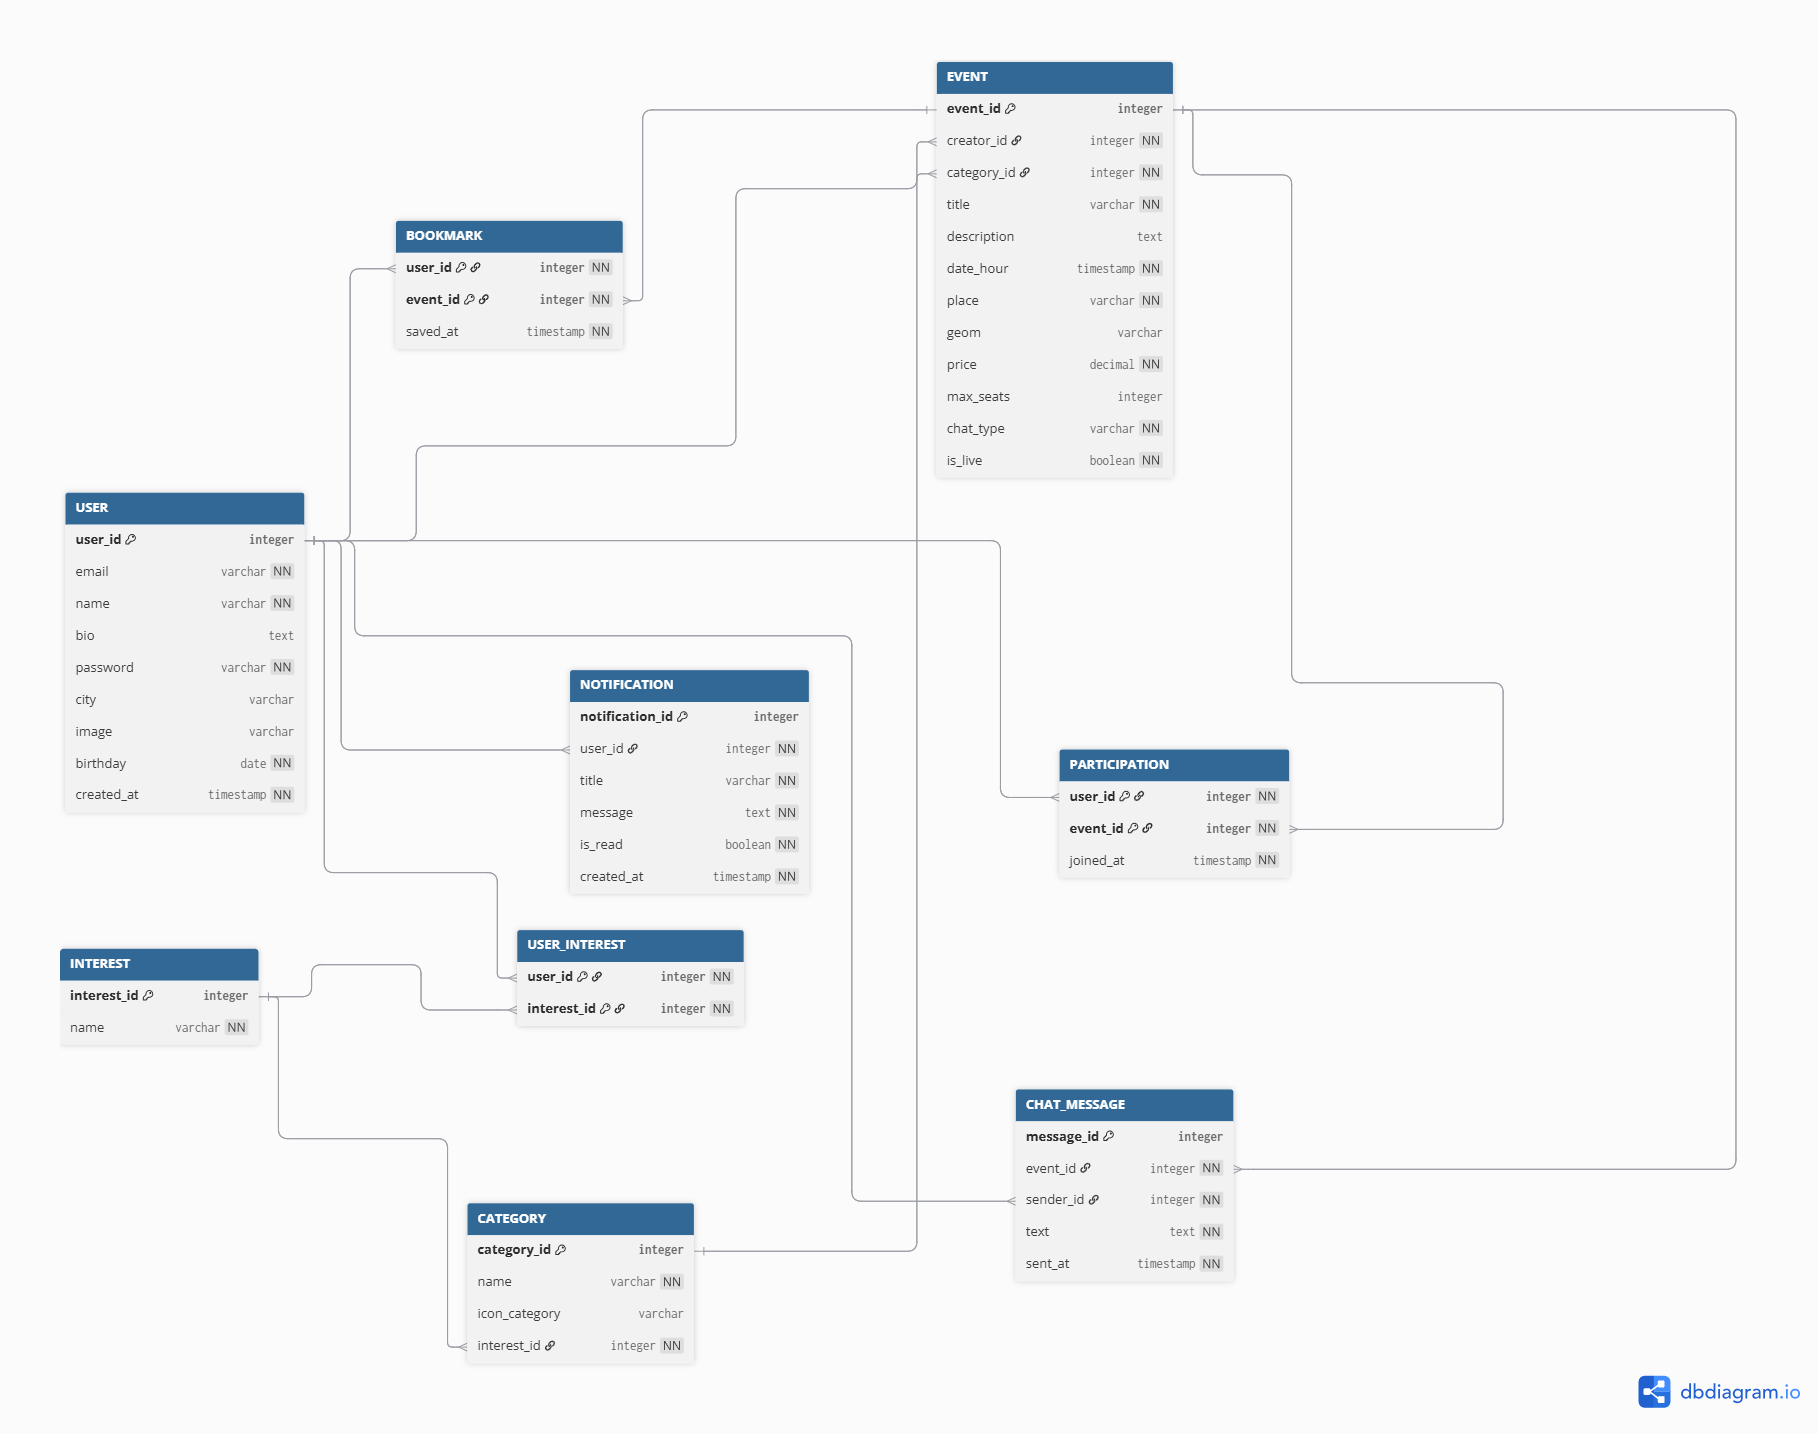
\includegraphics[width=\textwidth]{images/schema-er.png}

\end{document}
    